\lesson{Qualtitative Changes in Equilibrium Systems}
\subsection{Le Chatelier's Principle}
When a chemical system at equilibrium is disturbed by a change in property, the system adjusts
in a way that opposes the change.
\begin{bulleted-list}
    \item \textbf{Equilibrium shift:} movement of a system at equilibrium, resulting in a change
        in the concentrations of reactants and products
    \item Keep in mind that any increase/decrease in concentration is \textbf{gradual}
\end{bulleted-list}

\subsection{Le Chatelier's Principle and Concentration Changes}
\begin{bulleted-list}
    \item In most industrial chemical processes, we want to ensure that equilibrium is not achieved.
        That is, the reverse reaction is not allowed to occur, for maximum efficiency and profit.
        For instance, the synthesis of ammonia in the Haber process
    \item To ensure the maximum efficiency, reactants are constantly added while products are
        simultaneously removed to utilize Le Chatelier's Principle in order to minimize the reverse
        reaction
    \item When you add particles to a reaction system, the rates at the new equilibrium state will
        be greater than before, because the system now contains a large number of particles. Likewise,
        if particles were removed, the rates at the new equilibrium state will be less than before
\end{bulleted-list}

\begin{figure}[ht!]
    \centering
    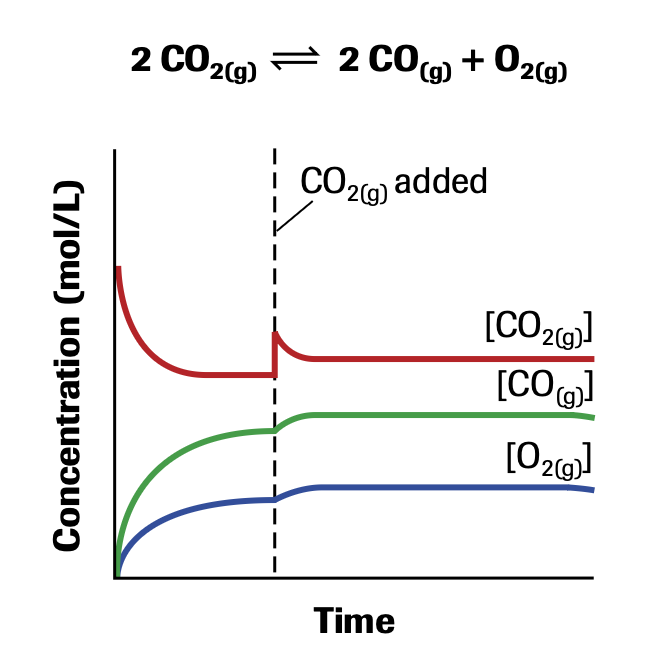
\includegraphics[width=0.4 \textwidth]{../figures/le-chateliers-principle-1.png}
    \caption{In this case, because reactants are being added, to achieve equilibrium,
    there will be a shift to the right to produce more products. This results in a concentration
    increase (till eventual decrease until equilibrium) in [$\ch{CO2_{(g)}}$] and a slight increase
    in [$\ch{CO_{(g)}}$] and [$\ch{O2_{(g)}}$]. Initially, the forward reaction rate is significantly
    faster than the reverse reaction rate, until they eventually equal once they reach a state of
    equilibrium once the reverse reaction rate begins to speed up.}
\end{figure}

\begin{figure}[ht!]
    \centering
    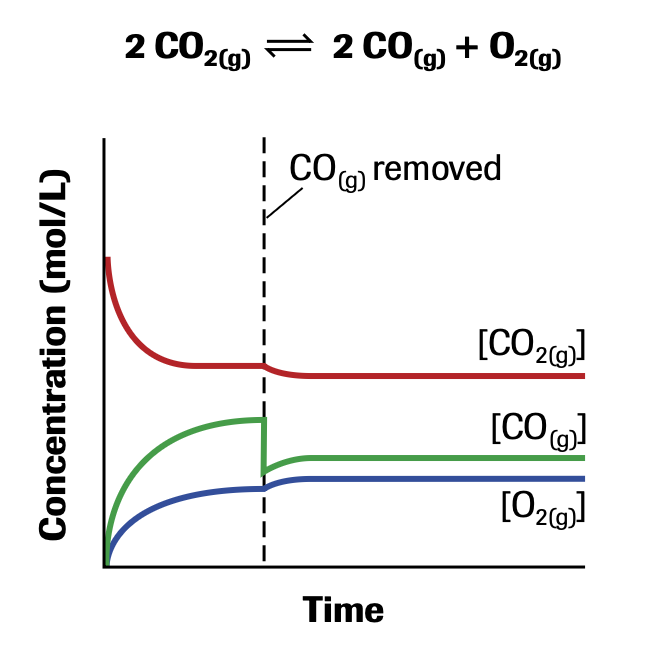
\includegraphics[width=0.4 \textwidth]{../figures/le-chateliers-principle-2.png}
    \caption{In this case, because products are being removed, to achieve equilibrium,
    there will be a shift to the right to produce more products. This results in a concentration
    decrease in [$\ch{CO2_{(g)}}$] and a slight increase in [$\ch{CO_{(g)}}$] and [$\ch{O2_{(g)}}$].
    Initially, the forward reaction rate is significantly faster than the reverse reaction rate, 
    until they eventually equal once they reach a state of equilibrium once the reverse reaction rate 
    begins to speed up.}
\end{figure}

\begin{figure}[ht!]
    \centering
    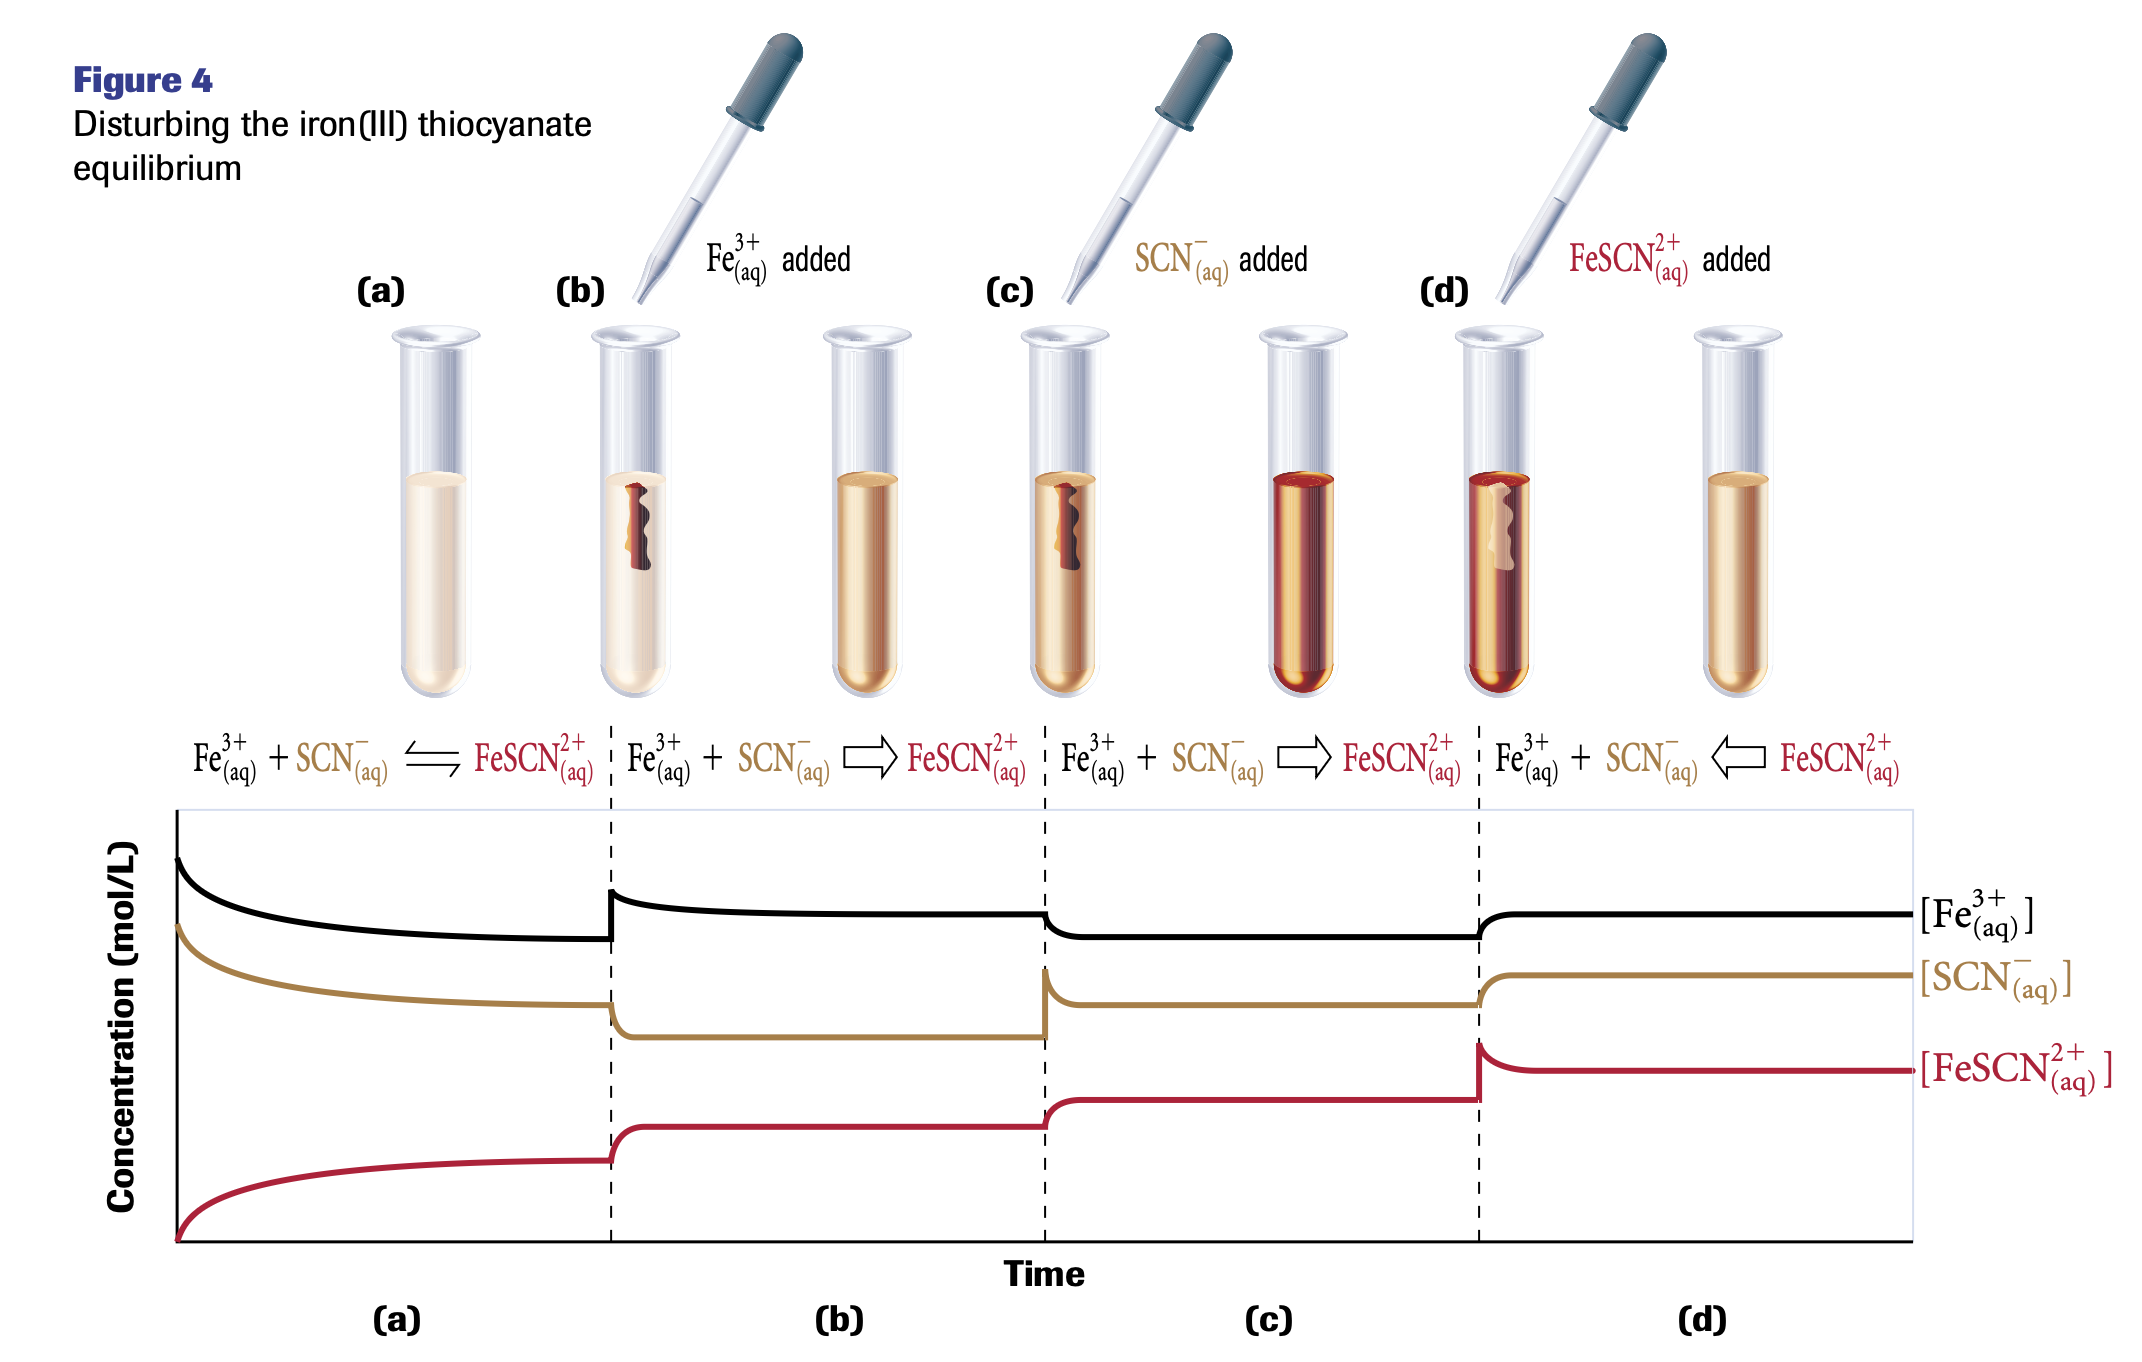
\includegraphics[width= \textwidth]{../figures/iron-3-thiocyanate-equilibrium-shift.png}
    \caption{An example of the effects of concentration change on equilibrium shift.}
\end{figure}

\subsection{Le Chatelier's Principle and Temperature Changes}
The two types of reactions to consider are endothermic and exothermic reactions
\begin{align*}
    \text{endothermic reaction: }&\text{reactants}+\text{energy}\rightleftharpoons \text{products}\\
    \text{exothermic reaction: }&\text{reactants}\rightleftharpoons \text{products}+\text{energy}
\end{align*}
\begin{bulleted-list}
    \item Energy can be added or removed to a system by heating or cooling the container. The
        equilibrium shifts, according to Le Chatelier's Principle, to minimize the changes
    \item If the system is \textbf{cooled}, the system tries to \textbf{warm itself up} by shifting
        the equilibrium in a direction that produces heat. If heat is added, the equilibrium
        position will shift such that heat is absorbed by the system
    \item For instance, in the decomposition of dinitrogen tetroxide
        \[
            \ch{N2O4_{(g)}}+\text{energy}\rightleftharpoons2 \ch{NO2_{(g)}}
        \]
        When the system at equilibrium is heated, the reaction shifts to the right, increasing
        the concentration of $\ch{NO2_{(g)}}$. This is made visible by the intensification of
        the reddish-brown colour. You can almost think of energy as a \textbf{chemical entity}
        partaking in the reaction
\end{bulleted-list}

\begin{figure}[ht!]
    \centering
    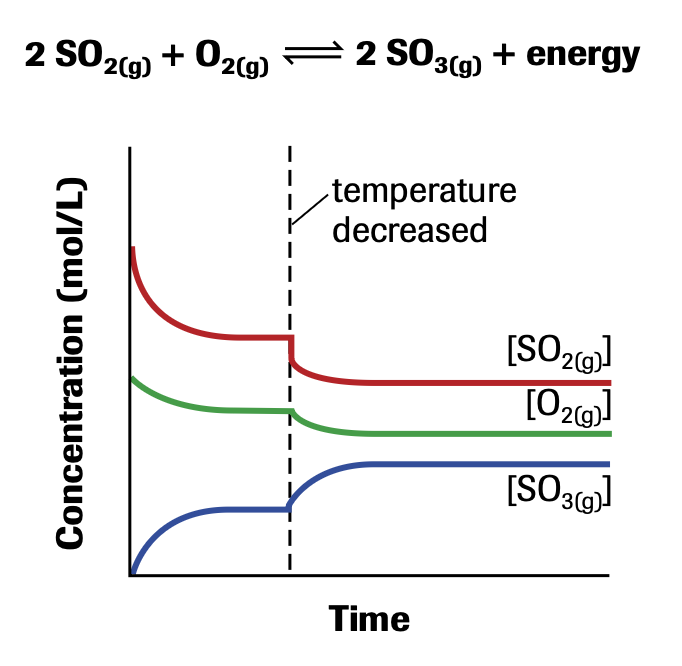
\includegraphics[width=0.4 \textwidth]{../figures/sulfur-trioxide-synthesis-equilibrium-shift.png}
    \caption{In this example, when the temperature is cooled, the system will counteract this change
    according to Le Chatelier's Principle by producing more heat. Thus, a right shift is observed by
    increasing the products via the consumption of reactants. Note that the forward rate is faster
    than the reverse rate initially, so that the system can produce more heat to counteract the
    decrease in temperature until equilibrium is achieved.}
\end{figure}

\begin{important}
    Temperature change is the only factor that will \textbf{change the equilibrium constant value}.
    This is because the equilibrium constant depends on the fact that the closed system has constant
    temperature and pressure.
\end{important}

\begin{figure}[ht!]
    \centering
    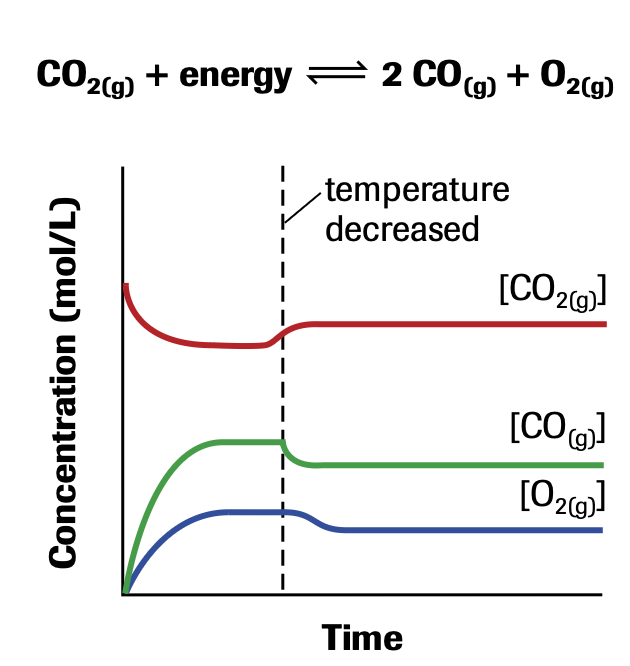
\includegraphics[width=0.4 \textwidth]{../figures/carbon-dioxide-decomposition-equilibrium-shift.png}
    \caption{In this example, when the temperature is cooledm the system will counteract this change
    by consuming less heat. Thus, a left shift is observed. Note that the reverse rate is faster than
    the forward rate initially, so that the system consumes less heat to counteract the decrease in 
    temperature until equilibrium is achieved.}
\end{figure}

\subsection{Le Chatelier's Principle and Gas Volume Changes}
\begin{bulleted-list}
    \item According to Boyle's Law, the volume and pressure are inversely proportional. That is,
        if the volume decreases by half, the pressure increases by a factor of two
    \item Changing the volume of any equilibrium system \textbf{may} cause a shift in the equilibrium.
        If all the reactants and products are aqeuous, then the shift in equilibrium is negligible.
        However, if there are chemical entities in the gaseous state, then a shift in equilibrium
        will be observed
    \item For instance, consider $\ch{N2_{(g)}}+\ch{3H2_{(g)}}\rightleftharpoons \ch{2NH3_{(g)}}$.
        On the reactants side, there are a total of 4 moles molecules, while on the product side, 
        there are a total of 2 moles of molecules. When there is an increase in pressure, Le Chatlier's
        Principle suggests that the system will counteract the increase in pressure by reducing
        the pressure. In this case, the equilibrium will shift to the right, since there will be
        less moles of molecules in the system
    \item A system with equal number of gas molecules on each side of the equation will not have
        an equilibrium shift
    \item Particles in the \textbf{solid, liquid, or aqueous state} are not of significance when it comes
        to determining equilibrium shift. This is because substances in these condensed states are
        virtually incompressible, and so reactions involving them cannot conteract pressure change
    \item Kinetic theory explains the effects of a decrease in volume by assuming that both the
        forward and reverse reaction rates increase because the concentrations (partial pressures)
        of reactants and products increase. However, the forward reaction rate increases more than
        the reverse reaction rate because there are more particles involved in the forward reaction.
        The shift causes concentration changes that eventually increase the reverse rate and decrease
        the forward rate until they become equal
\end{bulleted-list}

\begin{figure}[ht!]
    \centering
    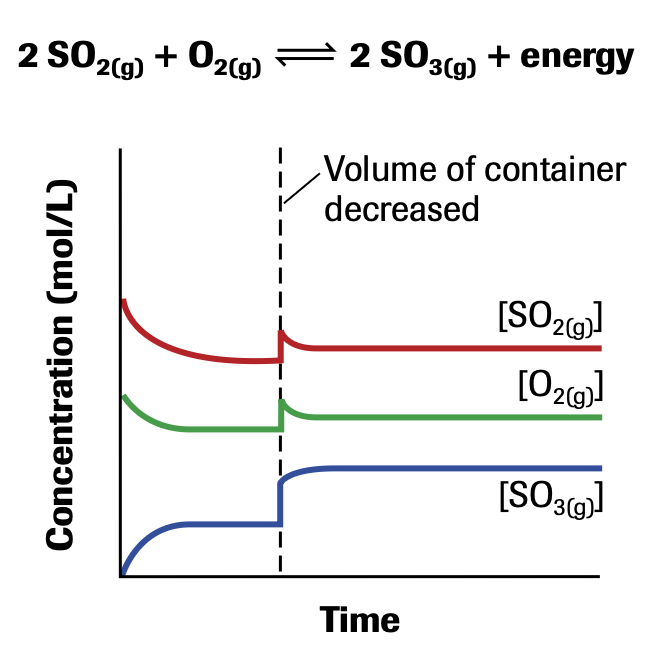
\includegraphics[width=0.4 \textwidth]{../figures/sulfur-trioxide-synthesis-equilibrium-change-gas.png}
    \caption{The equilibrium is disturbed by a decrease in volume. The equilibrium shifts forward
    to counteract the increase in pressure.}
\end{figure}

\subsection{Common Ion Effect}
The solubility of an ionic solids dissolved in pure water differs from a solution that contains
a common ion to the ionic solid. For instance, consider dissolving sodium chloride in pure water
versus dissolving it in sodium hydroxide solution. In the latter case, there is already an
abundance of sodium ions before adding in the sodium chloride, which will affect the equilibrium
position.

\begin{important}
    Regardless of whether there are pre-existing common ions in the solution or not, the solubility
    product of the salt, $K_\mathrm{sp}$, remains the same. The $K_\mathrm{sp}$ expression does
    not specify ions FROM that specific salt, but rather the entire concentration of ions.
\end{important}

The common ion effect is the expression used to describe the lowering of the solubility of a salt
because the solvent into which it is being dissolved already contains ion(s) common to the salt.

\subsection{Changes That Do Not Affect The Position of Equilibrium Systems}
\begin{bulleted-list}
    \item \textbf{Adding Catalysts}
        \begin{bulleted-list}
            \item The prescence of a catalyst in a chemical reaction system lowers the activation
                energy for both forward and reverse reactions by an equal amount, so the equilibrium
                state is established much quicker but at the \textbf{same position} as it would without
                a catalyst
            \item Forward and reverse reaction rates are increased equally
            \item The value of catalysts in industrial processes is to decrease the time required
                for equilibrium shifts to occur, allowing a more rapid overall production of the
                desired product
        \end{bulleted-list}
    \item \textbf{Adding Inert Gases}
        \begin{bulleted-list}
            \item Adding inert gases, such as noble gases, which will not partake in the reaction
                of the system, does not affect the equilibrium position
            \item It may, however, affect the speed at which the equilibrium position is established,
                similar to the catalyst
            \item According to kinetic theory, the prescence of inert gas changes the probability
                of a successful collision for both the reactants and products equally,
                resulting in no shift in the equilibrium system
        \end{bulleted-list}
\end{bulleted-list}

% lcp presentation
% \begin{table}[!ht]
%     \centering
%     \setlength{\tabcolsep}{12pt}      % column spacing
%     \renewcommand{\arraystretch}{1.2} % row spacing
%     \arrayrulecolor{black}            % table border color
%     \begin{tabular}{l l}
%         $\ch{CO_{(g)}}+\ch{2H2_{(g)}}\rightleftharpoons \ch{CH3OH_{(g)}}$ & $\Delta H_r^{\circ}=-91\,\si{kJ.mol^{-1}}$ \\
%         $\ch{CO_{(g)}}+\ch{H2O_{(g)}}\rightleftharpoons \ch{CO2_{(g)}}+\ch{H2_{(g)}}$ & $\Delta H_r^{\circ}=-41\,\si{kJ.mol^{-1}}$ \\
%         $\ch{CO2_{(g)}}+\ch{3H2_{(g)}}\rightleftharpoons \ch{CH3OH_{(g)}}+\ch{H2O_{(g)}}$ & $\Delta H_r^{\circ}=-50\,\si{kJ.mol^{-1}}$
%     \end{tabular}
% \end{table}
%
% \[
%     \ch{A_{(g)}}+\ch{B_{(g)}}\rightleftharpoons \ch{C_{(g)}}
% \]
% \[
%     K_\mathrm{eq}=\frac{P_\mathrm{C}}{P_\mathrm{A}\cdot P_\mathrm{B}}
% \]
% \begin{align*}
%     P_\mathrm{A}&=x_\mathrm{A}\cdot P_\mathrm{total}\\
%     P_\mathrm{B}&=x_\mathrm{B}\cdot P_\mathrm{total}\\
%     P_\mathrm{C}&=x_\mathrm{C}\cdot P_\mathrm{total}
% \end{align*}
% \[
%     K_\mathrm{eq}=\frac{P_\mathrm{C}}{P_\mathrm{A}\cdot P_\mathrm{B}}=\frac{1}{1\cdot 1}=1
% \]
% \begin{align*}
%     x_\mathrm{A}&=\frac{n_\mathrm{A}}{n_\mathrm{total}}\\
%     x_\mathrm{B}&=\frac{n_\mathrm{B}}{n_\mathrm{total}}\\
%     x_\mathrm{C}&=\frac{n_\mathrm{C}}{n_\mathrm{total}}\\
% \end{align*}
% \[
%     P_\mathrm{A}=1\,\si{atm},\,P_\mathrm{B}=1\,\si{atm},\,P_\mathrm{C}=1\,\si{atm},\,P_\mathrm{total}=3\,\si{atm}
% \]
% \[
%     n_\mathrm{I}=1\,\si{mol},\,P_\mathrm{I}=1\,\si{atm},\,P_\mathrm{total\,(new)}=4\,\si{atm}
% \]
% \begin{align*}
%     P_\mathrm{A\,(new)}&=x_\mathrm{A\,(new)}\cdot P_\mathrm{total\,(new)}\\
%                 &=\frac{1\,\si{mol}}{4\,\si{mol}}\cdot (4\,\si{atm})\\
%                 &=1\,\si{atm}\\
%                 &=P_\mathrm{A}
% \end{align*}
% \begin{align*}
%     Q&=\frac{P_\mathrm{C\,(new)}}{P_\mathrm{A\,(new)}\cdot P_\mathrm{B\,(new)}}\\
%                   &=\frac{P_\mathrm{C}}{P_\mathrm{A}\cdot P_\mathrm{B}}\\
%                   &=\frac{1}{1\cdot 1}\\
%                   &=1\\
%                   &=K_\mathrm{eq}
% \end{align*}
% \[
%     \ch{A_{(g)}}+\ch{B_{(g)}}\rightleftharpoons \ch{C_{(g)}}+\ch{D_{(g)}}
% \]
% \[
%     \ch{C_{(g)}}\rightleftharpoons \ch{A_{(g)}}+\ch{B_{(g)}}
% \]
%
% \begin{align*}
%     n_\mathrm{A}&=1\,\si{mol}\\
%     n_\mathrm{B}&=1\,\si{mol}\\
%     n_\mathrm{C}&=1\,\si{mol}\\
%     n_\mathrm{D}&=1\,\si{mol}\\
%     V&=2\,\si{L}
% \end{align*}
%
% \begin{align*}
%     [\mathrm{A]}&=\frac{1}{2}\,\si{mol.L^{-1}}\\
%     [\mathrm{B}]&=\frac{1}{2}\,\si{mol.L^{-1}}\\
%     [\mathrm{C}]&=\frac{1}{2}\,\si{mol.L^{-1}}\\
%     [\mathrm{D}]&=\frac{1}{2}\,\si{mol.L^{-1}}\\
% \end{align*}
%
% \begin{align*}
%     K_\mathrm{eq}&=\frac{[\mathrm{C}]}{[\mathrm{A}][\mathrm{B}]}\\
%                  &=\frac{\frac{1}{2}}{(\frac{1}{2})(\frac{1}{2})}\\
%                  &=2
% \end{align*}
%
% \[
%     n_\mathrm{I}=1\,\si{mol},\,V_\mathrm{new}=3\,\si{L}
% \]
% \begin{align*}
%     [\mathrm{A]}_\mathrm{new}&=\frac{1}{3}\,\si{mol.L^{-1}}\\
%     [\mathrm{B}]_\mathrm{new}&=\frac{1}{3}\,\si{mol.L^{-1}}\\
%     [\mathrm{C}]_\mathrm{new}&=\frac{1}{3}\,\si{mol.L^{-1}}\\
%     [\mathrm{D}]_\mathrm{new}&=\frac{1}{3}\,\si{mol.L^{-1}}
% \end{align*}
%
% \begin{align*}
%     Q&=\frac{[\mathrm{C}]_\mathrm{new}}{[\mathrm{A}]_\mathrm{new}[\mathrm{B}]_\mathrm{new}}\\
%                  &=\frac{\frac{1}{3}}{(\frac{1}{3})(\frac{1}{3})}\\
%                  &=3\\
%     Q&>K_\mathrm{eq}
% \end{align*}
%
% \begin{align*}
%     K_\mathrm{eq}&=\frac{[\mathrm{A}][\mathrm{B}]}{[\mathrm{C}]}\\
%                  &=\frac{(\frac{1}{2})(\frac{1}{2})}{\frac{1}{2}}\\
%                  &=\frac{1}{2}
% \end{align*}
%
% \begin{align*}
%     Q&=\frac{[\mathrm{A}]_\mathrm{new}[\mathrm{B}]_\mathrm{new}}{[\mathrm{C}]_\mathrm{new}}\\
%      &=\frac{(\frac{1}{3})(\frac{1}{3})}{\frac{1}{3}}\\
%      &=\frac{1}{3}\\
%     Q&<K_\mathrm{eq}
% \end{align*}
%
% \begin{align*}
%     K_\mathrm{eq}&=\frac{[\mathrm{C}][\mathrm{D}]}{[\mathrm{A}][\mathrm{B}]}\\
%                  &=\frac{(\frac{1}{2})(\frac{1}{2})}{(\frac{1}{2})(\frac{1}{2})}\\
%                  &=1
% \end{align*}
%
% \begin{align*}
%     Q&=\frac{[\mathrm{C}]_\mathrm{new}[\mathrm{D}]_\mathrm{new}}{[\mathrm{A}]_\mathrm{new}[\mathrm{B}]_\mathrm{new}}\\
%                  &=\frac{(\frac{1}{3})(\frac{1}{3})}{(\frac{1}{3})(\frac{1}{3})}\\
%                  &=1\\
%                  &=K_\mathrm{eq}
% \end{align*}
% \begin{align*}
%     \ch{CH4_{(g)}}+\ch{2H2O_{(g)}}\rightleftharpoons \ch{CO2_{(g)}}+\ch{4H2_{(g)}}
% \end{align*}
